\documentclass[10pt]{article}
\usepackage{NotesTeXV3,lipsum}
%\usepackage{showframe}

\renewcommand{\vec}{\mathbf}
\begin{document}
	\title{{Quantum Mechanics II: PHYS 312}\\{\normalsize{\itshape 
				typed revision
	}}}
	\author{Ahmed Saad Sabit}
	\affiliation{
	Sophomore at Rice University\\
	\href{https://kneardhead.github.io/}{Website}\\
	}
	\emailAdd{ahmedsaadsabit@rice.edu}
	\maketitle
	\newpage
	\pagestyle{fancynotes}

\part{Methodology}
\section{Reading this handout} 
What I am going to do is that
\begin{prob}
	This is a problem statement.
\end{prob}
\begin{solu}
	This is a solution statement. 
\end{solu}
\begin{margintable}
	\[
	\vec{E} = p^2 c^2 + m^2 c^{4}
	\] 
\end{margintable}
\begin{definition}
	This is a definition. 
\end{definition}
\begin{fact}
This is a fact. By fact I mean it's a derivative of Definition.
\end{fact}



\newpage
\part{Perturbation Theory: \\Examples} 
\section*{Zeeman Effect without Spin} 
This is an easier version of the problem where we ignore spin. When we do consider spin eventually, the problem is then called Spin-Orbit Coupling [see section ??]. 

\subsection*{Zeeman Effect} 
We know from our study of Perturbation theory that \emph{degeneracies appear because of some symmetry.} The $n$ energy levels of atom are all degenerate. But turning the Magnetic Field On would break the symmetry and we should expect the degenerate energy levels to be no more degenerate: which means we should have different energy levels within $n$ orbit now. 

\subsection*{Handwavy Derivation of $H'$ }
To do perturbation theory we first need the Perturbed Hamiltonian term to add to the unperturbed Hamiltonian. As we turn on the Magnetic Field (or slowly ramp it up from zero, which is probably how it should be done \textcolor{red}{ask professor}) that adds to the effective energy of the atom because a ``spinning electron" has an effective magnetic dipole moment. 

\[
\vec{M} = \text{(current)} \times \text{(area of electron path loop)} * \text{unit vector perp to loop area}
\] 
We get
\[
\vec{M} = - \frac{ev}{2 \pi r} \cdot  \pi r^2  \hat{n} = - \frac{evr}{2} \hat{n}
\]
\newcommand{\hb}{\hbar} 
Using $|\vec{L}| = \mu r v$ where $\mu$ is the reduced mass
\[
\vec{M} = - \frac{e \vec{L}}{2 \mu} = - \left(\frac{e}{2 m_e} \hb \right) \frac{\vec{L}}{\hb} \implies 
\hat{\mathbf{M}} = - \mu_B \frac{\hat{\mathbf{L}}}{\hb}
\]
and at the end we invoked that $\vec{L}$ is actually a Quantum Mechanical operator.
Energy of the magnetic dipole in a given $\vec{B}$ field 
\[
	\hat{H}' = - \hat{\mathbf{M}}\cdot \vec{B}
\] 
\begin{margintable} \textbf{Note:}
	Please note that in fact the proper treatment gives an extra term  proportional to $B^2$ but this is comparable to second order effects from $\hat{\vec{H}}'$ and we will only analyze the first order effects. 
\end{margintable}
Thus we find 
\[
\boxed{
\hat{\vec{H}} ' = \frac{\mu_B}{\hb} \hat{\vec{L}}\cdot \vec{B}
}
\] 


\subsection*{First order Perturbation Theory on Hydrogen Ground State} 
The ground state is $n = 0, l = 0, m = 0$ and using the equation for the first order energy perturbation for this given state
\[
	\bra{\psi_{100}} \hat{L_z} \ket{\psi_{100}} =  \bra{\psi_{100}} \left(m \ket{\psi_{100}}\right) = 0 \tag{$m$ is zero}	
\] 

First order perturbation to state vector 
\[
	\ket{\psi_{100}}^{(1)} = \frac{\mu_B B}{\hb}
	\sum_{j \neq \text{g.s}}^{\text{all state}} \frac{\bra{j} \hat{L}_z \ket{\psi_{100}}}{E_{\text{g.s}}^{(0)} - E_j^{(0)}} \propto m =0
\] 	
Here $g.s$ means ground state and because of the same reason that $\hat{L}_z$ brings out the $m$ from $\psi_{100}$ we have the whole thing go to zero.

\subsection*{First Order Perturbation Theory on Hydrogen First Excited State}
The given unperturbed states for $n = 2$ are 
\begin{align*}
	\psi_{200}, \psi_{211}, \psi_{210}, \psi_{21 \bar{1}}  (= \psi_{21-1} )
\end{align*}
I shifted the minus sign of $-1$ in the last state above because $21 \bar{1}$ looks more aesthetic than $21-1$. This is also something done in miller indices to explain crystallographic structures.

The given states in $n=2$ are 4 fold degenerate (which means there are 4 states that have the same Energy, also meaning same Eigenvalue). 

Let's construct the matrix elements of $H'$ in the basis of the given unperturbed energy eigenkets, 

\[
	\hat{\vec{H}}' = 
\begin{pmatrix}
\langle 2, 0, 0 | H' | 2, 0, 0 \rangle & \langle 2, 0, 0 | H' | 2, 1, -1 \rangle & \langle 2, 0, 0 | H' | 2, 1, 0 \rangle & \langle 2, 0, 0 | H' | 2, 1, 1 \rangle \\
\langle 2, 1, -1 | H' | 2, 0, 0 \rangle & \langle 2, 1, -1 | H' | 2, 1, -1 \rangle & \langle 2, 1, -1 | H' | 2, 1, 0 \rangle & \langle 2, 1, -1 | H' | 2, 1, 1 \rangle \\
\langle 2, 1, 0 | H' | 2, 0, 0 \rangle & \langle 2, 1, 0 | H' | 2, 1, -1 \rangle & \langle 2, 1, 0 | H' | 2, 1, 0 \rangle & \langle 2, 1, 0 | H' | 2, 1, 1 \rangle \\
\langle 2, 1, 1 | H' | 2, 0, 0 \rangle & \langle 2, 1, 1 | H' | 2, 1, -1 \rangle & \langle 2, 1, 1 | H' | 2, 1, 0 \rangle & \langle 2, 1, 1 | H' | 2, 1, 1 \rangle
\end{pmatrix}
\] 

If you plug in the form of $H'$ here and solve each of the elements you will quickly realize only the diagonal terms remain with non-zero $m$. We end up solving 
\[
\hat{\vec{H}} ' = \frac{\mu_B B}{\hb} 
\begin{pmatrix} 0 & 0 & 0 & 0 \\ 
0 & \hb & 0 & 0 \\
0 & 0 & 0 & 0 \\ 
0& 0 & 0 & - \hb \end{pmatrix} 
\] 
\begin{figure}[H]
	\centering
	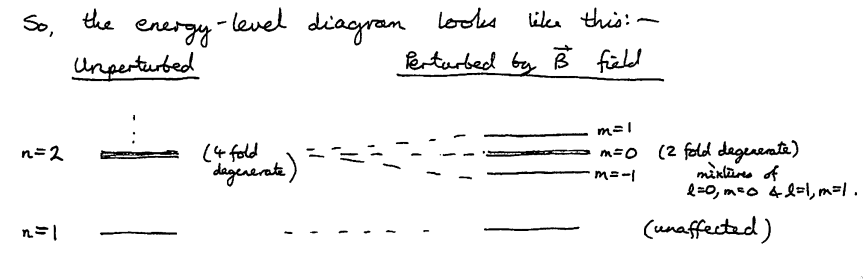
\includegraphics[width=1\textwidth]{./ss/m/1.png}
	\caption{./ss/m/1.png}
	\label{fig:-ss-m-1-png}
\end{figure}

We could try to compute the first order perturbation (or call correction) to the wavefunction but because the given $\ket{nlm}$ states are already diagonal in $\hat{\vec{H}}'$, they are already the eigenstates hence there are no terms. 















\section*{The Stark Effect} 
\[
\hat{\vec{H}}' = - \vec{p} \cdot \vec{E} =  - \left(- e \hat{\vec{r}}\right)\cdot \vec{E} = e \vec{E} \cdot  \hat{\vec{r}} \implies e |\vec{E}| r \cos \theta
\]
\subsection*{Perturbation for Ground State of Hydrogen} 
\[
	E^{(1)}_{g.s} = e E \bra{\psi_{100}} r \cos \theta \ket{\psi_{100}}
\] 
Like before I will come up with an operator method to do this later. But for now it's better for us to try solving this through integral wave formulation 
\begin{margintable}
	\[
	\int \mathrm{d} \phi = 2 \pi
	\] 
	\[
		\int_{0}^{\pi} \sin \theta \, d \theta = - \int_{1}^{-1} d (\cos \theta)
	\] 
	\[
	= \int_{-1}^{1} d (\cos \theta) 
	\] 
\end{margintable}
\begin{align*}
	E^{(1)}_{g.s} &= e E \bra{\psi_{100}} r \cos \theta \ket{\psi_{100}} \\ 
		      &= \int \mathrm{d} V \psi^{*}_{100} (\vec{r}) (r \cos \theta)  \\
		      &= \int r^2 \sin \theta \mathrm{d} \theta d \phi d r\,  \psi^{*}_{100} (\vec{r}) (r \cos \theta) 
		      \psi_{100}(\vec{r}) \\ 
		      &= 2 \pi \int d(\cos \theta ) dr \, r^3 \cos \theta \psi_{100}^{*} \psi_{100} \\
		      &= 2 \pi \int d(\cos \theta ) \cos \theta  \int dr \, r^3 \psi_{100}^{*} \psi_{100} \\
\end{align*}
The angular part of the integral can be solved by noticing that $\int_{-1}^{1} d(\cos \theta) $ is in even range while the integrand $\cos \theta$ is odd, so the integral is zero. Further rant about parity mentioned below

\subsection*{Parity} 
The parity operator $\hat{P}$ sends $\vec{r}$ to $- \vec{r}$. In cartesian 
\[
x_i \to  - x_i
\]  
And 
\begin{align*}
r \to  r \\ 
\theta \to  \pi - \theta \\ 
\phi \to  \phi + \pi 
\end{align*}
Parity operator twice is same as bringing back the original ket to where it was hence $\hat{\vec{P}}^2 = \hat{I}$. Thus the Eigenvalues of $\hat{\vec{P}}$ must be either $+1$ or $-1$. 

For eigenvalue $+1$ we have even parity, for $-1$ we have odd parity.

Hamiltonian of any spherically symmetric system commutes with $\hat{\vec{P}}$. One example being the unperturbed $H$-atom that commutes with the parity operator. It's eigenstates are also eigenstates of $\hat{\vec{P}}$.

Spherical Harmonics are Eigenstates of $\hat{\vec{P}}$, with Eigenvalues $(-1)^{l}$. So $l = 0,2,4, \ldots$ are even parity and $l = 1, 3, 5, \ldots$ are odd parity.

\begin{prob}Prove that parity eigenvalue of Spherical Harmonics is given by $(-1)^{l}$ 
	\end{prob} 
	\begin{solu}
		\begin{small} 
To explicitly compute the parity eigenvalues of the spherical harmonics \( Y_\ell^m(\theta, \varphi) \), we can analyze their behavior under the parity transformation, which inverts the spatial coordinates: \( \mathbf{r} \rightarrow -\mathbf{r} \). In spherical coordinates, this inversion corresponds to \( (\theta, \varphi) \rightarrow (\pi - \theta, \pi + \varphi) \).

The spherical harmonics are defined as:

\[ Y_\ell^m(\theta, \varphi) = N_\ell^m \, P_\ell^m(\cos \theta) \, e^{i m \varphi} \]

where \( N_\ell^m \) is a normalization constant, and \( P_\ell^m \) are the associated Legendre polynomials.

Under the parity transformation:

\[ Y_\ell^m(\pi - \theta, \pi + \varphi) = N_\ell^m \, P_\ell^m(\cos(\pi - \theta)) \, e^{i m (\pi + \varphi)} \]

Using the properties:

- \( \cos(\pi - \theta) = -\cos(\theta) \)
- \( e^{i m (\pi + \varphi)} = e^{i m \pi} \, e^{i m \varphi} = (-1)^m \, e^{i m \varphi} \)

we have:

\[ Y_\ell^m(\pi - \theta, \pi + \varphi) = N_\ell^m \, P_\ell^m(-\cos \theta) \, (-1)^m \, e^{i m \varphi} \]

The associated Legendre polynomials satisfy:

\[ P_\ell^m(-x) = (-1)^{\ell + m} \, P_\ell^m(x) \]

Applying this property:

\[ P_\ell^m(-\cos \theta) = (-1)^{\ell + m} \, P_\ell^m(\cos \theta) \]

Therefore:

\[ Y_\ell^m(\pi - \theta, \pi + \varphi) = N_\ell^m \, (-1)^{\ell + m} \, P_\ell^m(\cos \theta) \, (-1)^m \, e^{i m \varphi} = (-1)^\ell \, Y_\ell^m(\theta, \varphi) \]

This confirms that the parity eigenvalue of \( Y_\ell^m \) is \( (-1)^\ell \). Thus:

- For even \( \ell \) (e.g., \( \ell = 0, 2, 4, \ldots \)), \( Y_\ell^m \) has even parity and remains unchanged under inversion.
- For odd \( \ell \) (e.g., \( \ell = 1, 3, 5, \ldots \)), \( Y_\ell^m \) has odd parity and changes sign under inversion.

This explicit computation aligns with the general property that spherical harmonics \( Y_\ell^m \) have parity \( (-1)^\ell \).
\qedsymbol.
\end{small}
\end{solu}


\begin{prob}
	Take eigenket that is even, prove that $\bra{\text{even}}  \vec{r}  \ket{\text{even}} = 0$. Here an example of $\ket{\text{even}}$ can be $l = 0, 2, 4, \ldots$ spherical harmonics solution to Hydrogen Wavefunction.
\end{prob}
\begin{solu}
	\begin{small}
		In quantum mechanics, the parity operator \( \hat{P} \) reflects spatial coordinates through the origin, transforming \( \mathbf{r} \) into \( -\mathbf{r} \). A function \( f(\mathbf{r}) \) is said to have even parity if \( f(-\mathbf{r}) = f(\mathbf{r}) \) and odd parity if \( f(-\mathbf{r}) = -f(\mathbf{r}) \).

The position operator \( \mathbf{r} \) is a vector quantity and thus has odd parity:

\[ \hat{P} \mathbf{r} \hat{P}^{-1} = -\mathbf{r} \]

Consider a quantum state \( | \psi \rangle \) with even parity:

\[ \hat{P} | \psi \rangle = | \psi \rangle \]

The matrix element \( \langle \psi | \mathbf{r} | \psi \rangle \) represents the expectation value of the position operator in the state \( | \psi \rangle \). Applying the parity operator to this expression:

\[ \langle \psi | \mathbf{r} | \psi \rangle = \langle \psi | \hat{P}^{-1} \hat{P} \mathbf{r} \hat{P}^{-1} \hat{P} | \psi \rangle = \langle \psi | \hat{P}^{-1} (-\mathbf{r}) \hat{P} | \psi \rangle = -\langle \psi | \mathbf{r} | \psi \rangle \]

Here, we used the facts that \( \hat{P} | \psi \rangle = | \psi \rangle \) and \( \hat{P} \mathbf{r} \hat{P}^{-1} = -\mathbf{r} \). This leads to:

\[ \langle \psi | \mathbf{r} | \psi \rangle = -\langle \psi | \mathbf{r} | \psi \rangle \]

The only solution to this equation is:

\[ \langle \psi | \mathbf{r} | \psi \rangle = 0 \]

Thus, the expectation value \( \langle \psi | \mathbf{r} | \psi \rangle \) vanishes for a state \( | \psi \rangle \) with even parity. This result generalizes: the matrix element \( \langle \phi | \mathbf{r} | \psi \rangle \) is zero unless the states \( | \phi \rangle \) and \( | \psi \rangle \) have opposite parity. This is because \( \mathbf{r} \) has odd parity, and the integral of an odd function over all space is zero.

In summary, for an operator with odd parity (like \( \mathbf{r} \)), its expectation value in a state with even parity is zero due to the symmetry properties under spatial inversion. 
	\end{small}
\end{solu}

\begin{prob}
	Show that this same analysis holds for $\bra{\text{odd}} \vec{r} \ket{\text{odd}}$.
\end{prob}
\begin{solu}
	\begin{small}
		If both kets are odd-parity states, we can follow the same reasoning as before.

   The position operator \( \mathbf{r} \) has \textbf{odd parity}, meaning:  
   \[
   \hat{P} \mathbf{r} \hat{P}^{-1} = -\mathbf{r}
   \]

   Let \( | \psi \rangle \) be an odd-parity state, meaning:  
   \[
   \hat{P} | \psi \rangle = -| \psi \rangle
   \]

   Consider the matrix element \( \langle \psi | \mathbf{r} | \psi \rangle \). Applying the parity operator, we get:  
   \[
   \langle \psi | \mathbf{r} | \psi \rangle = \langle \psi | \hat{P}^{-1} \hat{P} \mathbf{r} \hat{P}^{-1} \hat{P} | \psi \rangle
   \]
   Since \( \mathbf{r} \) has odd parity and \( | \psi \rangle \) has odd parity:  
   \[
   \hat{P} \mathbf{r} \hat{P}^{-1} = -\mathbf{r}, \quad \hat{P} | \psi \rangle = -| \psi \rangle
   \]
   Therefore:  
   \[
   \langle \psi | \mathbf{r} | \psi \rangle = \langle \psi | (-\mathbf{r}) | \psi \rangle
   \]
   \[
   = -\langle \psi | \mathbf{r} | \psi \rangle
   \]

   The only way for this equation to be true is if  
   \[
   \langle \psi | \mathbf{r} | \psi \rangle = 0
   \]
   meaning the expectation value still vanishes. \qedsymbol.
	\end{small}
\end{solu}

Doing the same with \[
\bra{\text{even}} P P^{-1} \vec{r} P  P^{-1} \ket{\text{odd}} = \bra{\text{even}} \vec{r} \ket{\text{odd}} 
\] hence the different parity turns out not to be zero. 

From this we know that 
\[
	E^{(1)}_{\text{g.s}} = 
	\bra{\Psi_{100} } r \ket{\Psi_{100}} e E =0 
\] 
because of both kets being the same parity. 

Let's look at the next order correction 
\[
	E_\text{g.s}^{(2)} = \sum_{\text{other than } \psi_{100}}^{\text{all state}} 
	\frac{
		| \bra{\psi_{100}} \hat{z} \ket{\psi_{nlm}} | ^2 e ^2 E_z^2 
	}{E_{\text{gs}}^{(0)} - E_{n}^{(0)}}
\] 
Now either we have to evaluate the whole sum or use a clever trick that is supposedly included in the handout. It's shown that we get $- ( 9 / 4) \alpha_0^3 |\vec{E}|^2$ for the second order energy correction (or perturbation).  


\end{document}
